\section{Main results}\label{sec_main}

In case (i), we provide the exact asymptotics for both the bias and variance terms, together with almost sharp convergence rates. We will use these results to illustrate the effects of the \emph{bias-variance tradeoff} and \emph{varying sample sizes}. In case (ii), we will prove an exact asymptotic variance limit, and employ the result to show the intricate effect of the covariate shift. On the other hand, in case (ii), we will provide an estimate on the bias term, which becomes exact only when $n_1\gg p$. 


\subsection{Covariate shift}\label{sec_diff}

We begin by considering the covariate shift setting where both tasks have the same linear model but different population covariance matrices.
We show the exact asymptotic limit of the excess risk of the HPS estimator in the high-dimensional setting.

First, we consider the variance. Recall from equation \eqref{Lvar} that the variance equation is equal to $\sigma^2 \cdot \bigtr{\Sigma^{(2)} (\hat\Sigma(a))^{-1}}$.
In particular, the matrix $\hat{\Sigma}$ adds up both tasks' sample covariance matrices.
Thus, the expectation of $\hat{\Sigma}(a)$ is equal to a mixture of both tasks' population covariance matrices, with mixing proportions determined by their sample sizes.
Intuitively, the spectrum of $\hat{\Sigma}(a)^{-1}$ now not only depends on the sample sizes of both tasks, but also depends on how well ``aligned'' $\Sigma^{(1)}$ and $\Sigma^{(2)}$ are.
To capture this alignment quantitatively, we introduce the covariate shift matrix %(rescaled by $a$)
$$ M \define (\Sigma^{(1)})^{\frac 1 2}(\Sigma^{(2)})^{-\frac 1 2}.$$
Let $\lambda_1 \ge \lambda_2 \ge \dots\ge \lambda_p $ be the singular values of $M$ in descending order.
Our first main result is the following theorem on the variance limit, which characterizes the exact dependence of $L_{\var}(a)$ on the singular values of $M$.


\begin{theorem}[Variance asymptotics under covariate shift]\label{thm_main_RMT}
Under Assumption \ref{assm_big1} (recalling $\varphi > 4$), for any small constant $c>0$, there exists a high probability event $\Xi$, on which the following estimate holds for $L_{\var}(a)$ in \eqref{Lvar}:
	\begin{align}\label{lem_cov_shift_eq}
		\bigabs{L_{\var}(a)- \frac{\sigma^2}{n_1+n_2}\bigtr{  \frac{1}{\alpha_1 a^2\cdot M^\top M + \alpha_2}  }}
		\le \frac{(n_1+n_2)^{\frac 2{\varphi} - \frac 1 2 + c}}{p^{1/2}}\cdot\frac{p \sigma^2}{n_1+ n_2},
	\end{align}
	uniformly in all $a\in \R$. Here $(\alpha_1, \alpha_2)$ is the solution of the following system of equations
	\begin{align}
		\alpha_1 + \alpha_2 = 1- \frac{p}{n_1 + n_2}, \quad
		\alpha_1 + \frac1{n_1 + n_2}  \bigbrace{\sum_{i=1}^p \frac{(a \lambda_i)^2 \alpha_1}{(a \lambda_i)^2 \alpha_1 + \alpha_2}} = \frac{n_1}{n_1 + n_2}. \label{eq_a12extra}
	\end{align}
\end{theorem}
\todo{changed $a_1, a_2$ to $\alpha_1, \alpha_2$ since they conflict with $a$}

Equation \eqref{lem_cov_shift_eq} thus characterizes the variance of the HPS estimator, up to an error term on the order of $O\big(\frac{\sigma^2}{p^{-1/2}}\big)$ (recall that $\varphi > 4$, $c$ is an arbitrarily small constant, $\frac{p}{n_1+n_2} \in (2 {\tau}, \frac 2 {\tau})$).
Our result can be viewed as a generalization of the classical result in Lemma \ref{fact_tr} to the \textit{covariate shift} setting.
In particular, Lemma \ref{fact_tr} corresponds to a setting where the singular values $\lambda_1,\dots,\lambda_p$ are all equal to one, and $a = 1$. Then, the second part of equation \eqref{eq_a12extra} simplifies to
\[ \alpha_1 + \frac{p}{n_1 + n_2}\cdot \frac{\alpha_1}{\alpha_1 + \alpha_2} = \frac{n_1}{n_1 + n_2}. \]
By solving the above together with the first part of equation \eqref{eq_a12extra}, we obtain that
$$\alpha_1 = \frac{n_1}{n_1+n_2},\quad \alpha_2 = \frac{n_2-p}{n_1+ n_2}.$$
Plugging the above solutions back to the variance limit, we thus find that the limit is equal to
\begin{align}
    \frac{\sigma^2}{n_1 + n_2} \bigtr{\frac 1 {\alpha_1 M^{\top} M + \alpha_2}} &= \frac{\sigma^2}{n_1 + n_2} \frac{p}{\alpha_1 + \alpha_2} \tag{since the singular values of $M$ are equal to $1$} \nonumber \\
    &= \frac{\sigma^2}{n_1 + n_2} \cdot\frac{p (n_1 + n_2)}{n_1 + n_2 - p} \tag{applying $\alpha_1$ and $\alpha_2$ from above} \nonumber \\
    &= \frac{\sigma^2 p}{n_1 + n_2 - p}, \label{g_id}
\end{align}
which is precisely the limit in Lemma \ref{fact_tr}.
Additionally, the convergence rate in equation \eqref{lem_cov_shift_eq} matches the one in Lemma \ref{fact_tr} for this special case.
%With Assumption \ref{assm_big1},
%$$ \frac{\sigma^2}{n_1+n_2}\bigtr{  \frac{1}{a_1 M(a)^\top M(a) + a_2  }  } \sim \frac{p \sigma^2}{n_1+ n_2}.$$
%Hence the right-hand side of \eqref{lem_cov_shift_eq} is much smaller than this main term by a factor of $p^{-1/2} (n_1+n_2)^{-1/2+2/\varphi + c}$, which we believe to be sharp up to the $(n_1+n_2)^c$ factor. Lemma \ref{fact_tr} can be also regarded as a special case of Theorem \ref{thm_main_RMT}. %also extends  to the inverse of the sum of two sample covariance matrices.
The proof of Theorem \ref{thm_main_RMT}, which is based on recent developments in random matrix theory \cite{Anisotropic}, can be found in Section \ref{appendix RMT}.

Second, we consider the bias.
Note that the setting where $\beta_1 = \beta_2$ can be viewed as a special case of the random-effect model with $d = 0$, thus, assuming that $\norm{\beta_1}_2^2 \ge \sigma^2 / p^{1/2 - c_0}$ for a small constant $c_0 > 0$, we have that $\hat B_1 / \hat B_2$ is equal to $1$ plus lower-order terms that scale to zero as $p$ goes to infinity (see equation \eqref{hatw_add1} for the precise scaling).
In Proposition \ref{lem_hat_v}, we have seen that the global minimizer $\hat a$ is close to 1 up to a small error.
Thus, the bias equation $L_{\bias}(\hat B_1 / \hat B_2)$ is equal to $0$ plus the above lower-order terms.
We summarize this discussion in the following corollary:

\begin{corollary}[Excess risk of HPS under covariate shift]\label{cor_hps_cov}
    Under Assumption \ref{assm_big1}, suppose further that $\beta_1 = \beta_2$ and $\norm{\beta_1}^2_2 \ge \frac{\sigma^2}{p^{1/2 - c_0}}$ for a constant $c_0 > 0$.
    Then, for any constant $c > 0$, the following estimate on the excess risk of the HPS estimator holds w.h.p.
    \begin{align}
        \bigabs{L(\hat{\beta}_2^{\MTL}) - \frac{\sigma^2}{n_1 + n_2} \bigtr{\frac{1}{\alpha_1 M^{\top} M + \alpha_2}}}
        \le
        \OO\bigbrace{\frac{(n_1+n_2)^{\frac 2{\varphi} - \frac 1 2 + c}}{p^{1/2}}\cdot\frac{p \sigma^2}{n_1+ n_2}
        + p^{-c_0 + 2c}},
    \end{align}
    where $\alpha_1$ and $\alpha_2$ are the solutions of equation \eqref{eq_a12extra} after taking $a = 1$.
\end{corollary}


\begin{figure}[!t]
	\begin{subfigure}[b]{0.5\textwidth}
		\centering
		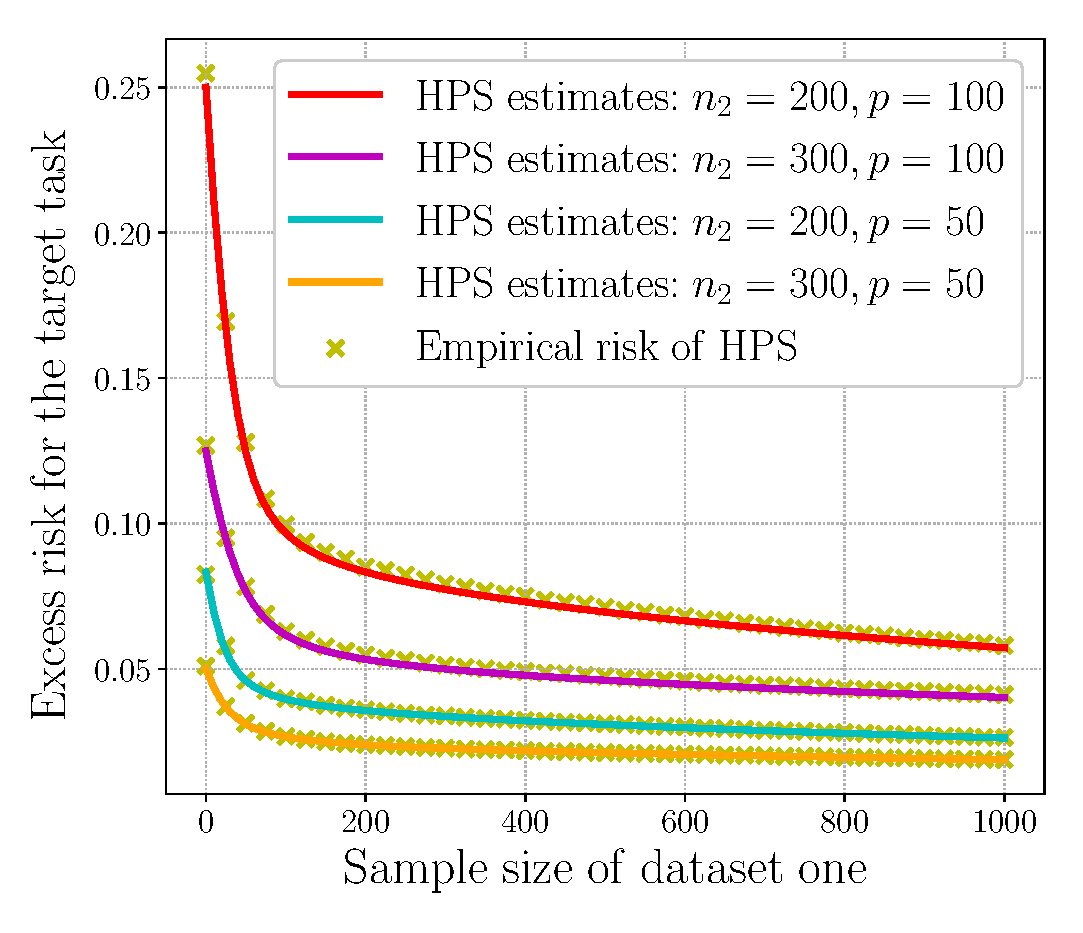
\includegraphics[width=0.9\textwidth]{figures/verify_covariate_shift.eps}
		\caption{Verify variance asymptotics in finite dimensions}
		\label{fig_sec3_verify_cov}
	\end{subfigure}
	\begin{subfigure}[b]{0.5\textwidth}
		\centering
		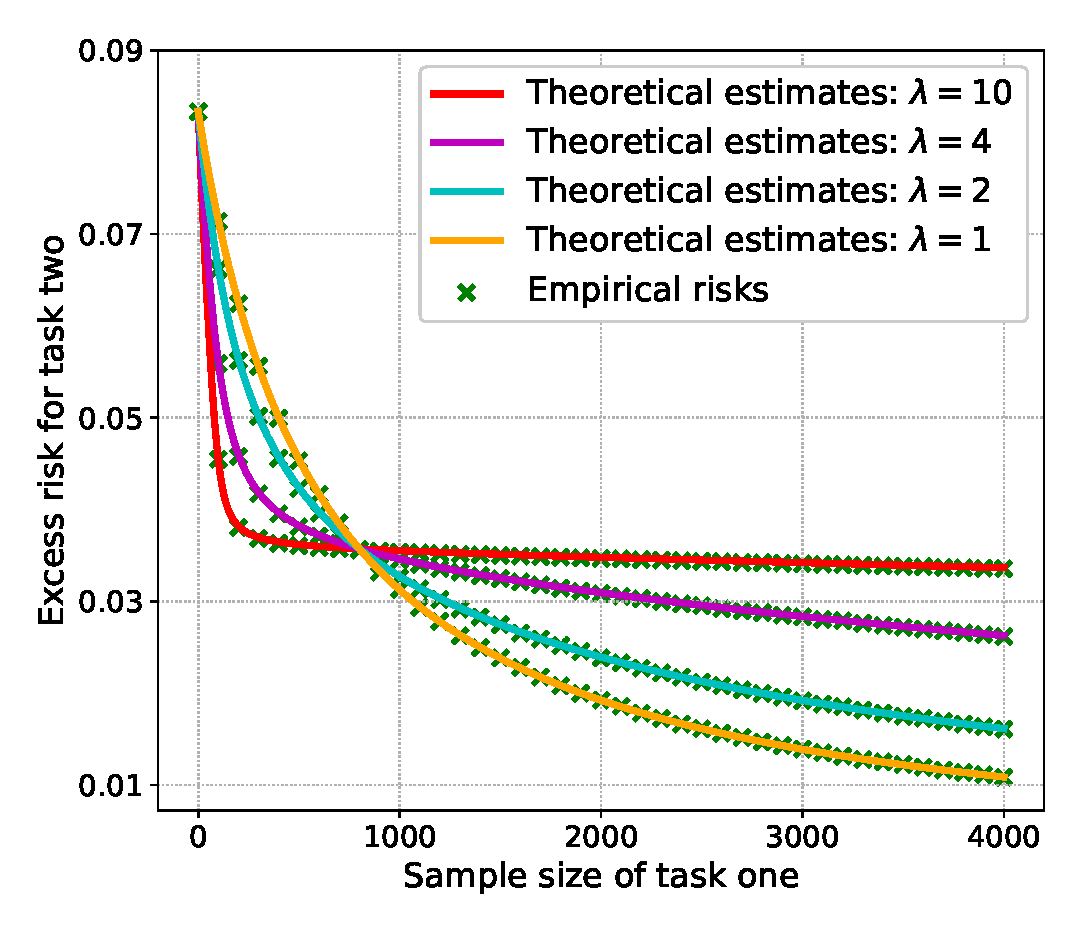
\includegraphics[width=0.9\textwidth]{figures/covariate_shift.eps}
		\caption{Sample size ratios vs. covariate shift}
		\label{fig_sec3_covariate}
	\end{subfigure}
	\caption{Figure \ref{fig_sec3_covariate}: we verify that Theorem \ref{thm_main_RMT} provides incredibly accurate estimates of the empirical variance under various finite sample sizes and dimensions.
	Figure \ref{fig_sec3_covariate}: We illustrate an intriguing dichotomy between covariate shift and sample size ratio: The dimension $p = 200$, $n_2 = 800$, and the noise variance $\sigma^2 = 1/4$.}
	\label{fig_sec31}
\end{figure}

\paragraph{Illustrative examples.}
Next, we illustrate the result of Corollary \ref{cor_hps_cov} in several examples.

\begin{example}[Does covariate shift help or hurt information transfer?]
    Our first example illustrates that the effect of covariate shift depends on the sample sizes of each dataset in an intricate manner.
    While the folklore belief is that transferring from a covariate-shifted distribution performs worse than an identical distribution, we show that, surprisingly, the former can sometimes outperform the latter.
    
    We first describe a setting for modeling covariate shift.
    Let $\cS$ be the set of positive definite matrices $M^{\top} M$ such that for $i = 1,2,\dots,\floor{\frac p 2}$, $\lambda_{p - i}  = \frac 1 {\lambda_i}$, where $\lambda_1 \ge \lambda_2 \ge \cdots \ge \lambda_p$ are the eigenvalues of $M$.
    Under this setting, we ask: suppose that the sample sizes $n_1$ and $n_2$ are both fixed, which $M$ provides the best ``transfer'' in the sense of HPS estimator's excess risk?
    We observe a dichotomy that depends on whether or not $n_1$ is greater than $n_2$.
    \begin{claim}[Covariate shift vs. sample size ratios]\label{claim_dichotomy}
        Let $g(M) = \frac{\sigma^2}{n_1 + n_2} \bigtr{\frac 1 {\alpha_1 M^{\top} M + \alpha_2}}$.
        Suppose that $n_1$ and $n_2$ are both fixed.
        Within the set of all possible covariate shift matrix $M\in\cS$, the following dichotomy holds:
        \begin{itemize}
	        \item If $n_1 \ge n_2$, then $g(M)$ is minimized in $\cS$ when $\lambda_i = 1$, for any $i = 1,\dots,p$.
	        \item If $n_1 < n_2$, then $g(M)$ is maximized in $\cS$ when $\lambda_i = 1$, for any $i = 1,\dots,p$.
        \end{itemize}
    \end{claim}

\begin{proof}
    We explain why the above dichotomy happens. We can write $g(M)$ for any $M \in \cS$ as
    $$g(M)=\frac{\sigma^2}{ n_1+n_2 }\sum_{i=1}^{p/2}\left( \frac{1}{\lambda_i^{2} a_1 + a_2} + \frac1{\lambda_i^{-2} a_1 + a_2} \right).$$
    When $M=\id_{p\times p}$, by the first equation of \eqref{eq_a12extra}, we have
    $$g(\id_{p\times p})=\frac{\sigma^2}{ n_1+n_2 }\sum_{i=1}^{p/2} \frac{2}{1-\gamma},$$
    where we abbreviate $\gamma:=p/(n_1+n_2)$. Then using $\alpha_1 + \alpha_2 = 1-\gamma$, through a direct calculation we find that
    \begin{align*}
        g(M) - g(\id_{p\times p})%&= \frac{\sigma^2 \gamma}{2(1-\gamma)} (\lambda^2-1)a_1\cdot \bigbrace{  \frac{1}{ -a_1(\lambda^2-1)+(1-\gamma)\lambda^2 } - \frac{1}{a_1(\lambda^2-1) + (1-\gamma)}} \\
        &= \frac{\sigma^2 }{ n_1+n_2-p} \sum_{i=1}^{p/2} \frac{(\lambda_i^2-1)^2 \alpha_1 \left[ \alpha_1 - \alpha_2\right] }{[\alpha_1 + \lambda_i^2 \alpha_2][\lambda_i^2 \alpha_1 + \alpha_2]} .
    \end{align*}
    %in this example is equal to
    %$\frac{p}{2(n_1 + n_2)} f(\lambda)$, where
    %\[ f(\lambda) = {(\lambda^{-2} a_1 + a_2)^{-1} + (\lambda^2 a_1 + a_2)^{-1}}. \]
    %Using the fact that $a_1 + a_2 = 1 - \frac{p}{n_1 + n_2}$, we can verify
    %\begin{align*}
    %	f(\lambda) - f(1) &= \left(\lambda^2 a_1 + \frac{n_1 + n_2 - p}{n_1 + n_2} - a_1\right)^{-1} \\
    %	&+ \left(\lambda^{-2} a_1 + \frac{n_1 + n_2 - p}{n_1 + n_2} - a_1\right)^{-1} \\
    %	&- \frac{2(n_1 + n_2)}{n_1 + n_2 - p} \\
    %	&= \left(2a_1 - \frac{n_1 + n_2-p} {n_1 + n_2 }\right)  g(\lambda, a_1), %\cdot (\lambda^2-1)^2
    %\end{align*}
    %\begin{align*}
    %	f(\lambda) - f(1) &= \left(2a_1 - \frac{n_1 + n_2-p} {n_1 + n_2 }\right)  g(\lambda, a_1), %\cdot (\lambda^2-1)^2
    %\end{align*}
    %where $g(\lambda, a_1) \ge 0$.
    %and can be derived from algebraic calculations (details omitted).
    We claim that $\alpha_1 > \alpha_2$ if and only if $n_1 > n_2$, which then explains the dichotomy.
    In fact, if $\alpha_1 > \alpha_2$, then the first part of equation \eqref{eq_a12extra} gives that $\alpha_1 > (1-\gamma)/2$.
    The second part of equation \eqref{eq_a12extra} gives that
    \begin{align*}
     \frac{n_1}{n_1 + n_2} &> \alpha_1 + \frac{1}{n_1+n_2} \sum_{i=1}^{p/2}\left(\frac{\lambda_i^2}{\lambda_i^2+1}+\frac{\lambda_i^{-2}}{\lambda_i^{-2}+1}\right) = \frac{1-\gamma}{2}+\frac{\gamma}{2}=\frac{1}{2}.
    \end{align*}
    %\begin{align*}
    % \frac{n_1}{n_1 + n_2} &=a_1 + \frac1{n_1 + n_2}\cdot \bigbrace{\sum_{i=1}^p \frac{\lambda_i^2 a_1}{\lambda_i^2 a_1 + a_2}} \\
    %	&> a_1 + \frac{p}{2(n_1+n_2)} \left(\frac{\lambda^2}{\lambda^2+1}+\frac{\lambda^{-2}}{\lambda^{-2}+1}\right) =\frac{1}{2}.
    %\end{align*}
    This is equivalent to $n_1>n_2$. The other direction follows from a similar argument. % Similarly, if $a_1<a_2$, equations  \eqref{eq_a12extra000} and  \eqref{eq_a12extra} give that $a_1 < \frac{n_1 + n_2-p}{2 (n_1 + n_2)}$ and $n_1<n_2$. Thus, we conclude that $f(\lambda) \ge f(1)$ if and only if $n_1 \ge n_2$.
    %\end{example}
\end{proof}

Figure \ref{fig_sec3_covariate} illustrates a special case where $\lambda_1 = \cdots = \lambda_{\floor{p /2}} = \lambda > 0$ for $M^{\top}M$ and the rest of the eigenvalues are all equal to $1 / \lambda$.
Thus, $\lambda > 0$ captures the degree of covariate shift: higher $\lambda$ implies worse covariate shift.
We observe that our theoretical estimates using Corollary \ref{cor_hps_cov} matches the empirical risks incredibly accurately.
As a result, we indeed observe the dichotomy shown in Claim \ref{claim_dichotomy}.
Furthermore, for higher $\lambda$, HPS' excess risk decreases slower--indicating a worse rate of ``transfer'' from task one. 
As a remark, the classical work of \citet{david2010impossibility} have likewise shown impossibility results for transfer learning under covariate shift in a classification setting.
By contrast, our analysis applies to a (high-dimensional) regression setting.
\end{example}


\begin{example}
Our second example illustrates that the effect of covariate shift worsens as the sample size of task one increases.
We consider a set of covariate shift matrices $M^{\top} M$ whose determinant are all equal to one, and the eigenvalues are bounded between $\tau^2$ and $1 / \tau^2$.
Let $\cS$ denote the set of $M\in\real^{p\times p}$ such that $M^{\top} M$ satisfies both conditions.
\begin{claim}[Identical covariance provides approximately optimal transfer under imbalanced dataset sizes]\label{prop_covariate}
    Recall that $g(M) = \frac{\sigma^2}{n_1 + n_2} \bigtr{\frac 1 {\alpha_1 M^{\top} M + \alpha_2}}$.
	We have the following result regarding $g(\id_{p \times p})$:
	\begin{align} g(\id_{p\times p}) \le \bigbrace{1+ {\frac{n_2}{\tau^2 n_1}  }} g(M), \text{ for any } M \in \cS. \label{eq_claim_id}
	\end{align}
\end{claim}
\begin{proof}
    We can write down the trace of $(\alpha_1 M^{\top} M + \alpha_2)^{-1}$ using the eigenvalues of $M^{\top} M$ as follows:
    \begin{align*}
        (\alpha_1 M^{\top} M + \alpha_2)^{-1} &= \sum_{i=1}^p \frac{1} {\alpha_1 \lambda_i^2 + \alpha_2} \\
        &\ge \sum_{i=1}^p \frac{1} {\alpha_1 \lambda_i^2 + \alpha_2 \cdot {\lambda_i^2} / {\tau^2}} \tag{since $\lambda_i \ge \tau$, for any $i$} \\
        &= \frac 1 {\alpha_1 + \alpha_2 / \tau^2} \sum_{i=1}^ p \frac 1 {\lambda_i^2} \\
        &\ge \frac 1 {\alpha_1 + \alpha_2 /\tau^2} p\cdot \bigbrace{\prod_{i=1}^p \frac 1 {\lambda_i^2}}^{1/ p} \tag{by the AM-GM inequality} \\
        &= \frac{p}{\alpha_1 + \alpha_2 / \tau^2} \tag{since $\prod_{i=1}^p \lambda_i^2 = \det(M^{\top} M) = 1$}
    \end{align*}
    Next, recall from equation \eqref{g_id} that
    $g(\id_{p\times p}) = \frac{\sigma^2 p}{n_1 + n_2 - p}$.
    Thus, equation \eqref{eq_claim_id} follows if we show that (after rearranging terms)
    \begin{align}
        \frac{n_1 + n_2}{n_1 + n_2 - p} \cdot \frac 1 {\alpha_1 + \frac{\alpha_2}{\tau^2}} \le 1 + \frac{n_2}{\tau^2 \cdot n_1}. \label{eq_claim_id_step}
    \end{align}
    From the second part of equation \eqref{eq_a12extra}, we have that
    \begin{align*}
        \frac{n_1} {n_1 + n_2} &= \alpha_1 + \frac 1 {n_1 + n_2} \bigbrace{\sum_{i=1}^p \frac{\lambda_i^2\alpha_1}{\lambda_i^2\alpha_1 + \alpha_2}} \\
        &< \alpha_1 + \frac p {n_1 + n_2}.
    \end{align*}
    Thus, $\alpha_1 > \frac{n_1 - p}{n_1 + n_2}$, which implies that $\alpha_2 < \frac{n_2}{n_1 + n_2}$.
    Hence, $\alpha_1 + \frac{\alpha_2}{\tau^2} = 1 - \frac{p}{n_1 + n_2} - \alpha_2 + \frac{\alpha_2}{\tau^2} \le 1 - \frac{p}{n_1 + n_2} + \frac{n_2}{n_1 + n_2} \frac 1 {\tau^2}$, which implies
    equation \eqref{eq_claim_id_step} by straightforward calculations.
    Thus, the proof is complete.
\end{proof}
As a corollary of Claim \ref{prop_covariate}, when $n_1$ is much larger than $n_2 / \tau^2$, the excess risk of HPS is approximately optimal in the set of all possible $M\in\cS$ when there is no covariate shift between dataset one and two.
\end{example}





\subsection{Model shift}\label{sec_sizeratio}

 In this subsection, we consider the setting where $X^{(1)}$ and $X^{(2)}$ are independent and have the same population covariance matrices $\Sigma^{(1)}=\Sigma^{(2)}$. However, the two tasks can have different sample sizes $n_1\ne n_2$. In this case, we can obtain the exact asymptotic limits of the bias term \eqref{Lbias} and the variance term \eqref{Lvar}. We will use these results to illustrate the effects of the bias-variance tradeoff and varying sample sizes on the performance of the $\MTL$ estimator.

\begin{theorem}[Excess risk of HPS under model shift]\label{cor_MTL_loss}
Under Assumption \ref{assm_big1}, suppose that $\Sigma^{(1)}=\Sigma^{(2)}$ and the entries of $Z^{(1)}$ and $Z^{(2)}$ are i.i.d. Gaussian random variables. Then for any small constant $\e>0$ and large constant $C>0$, there exists a high probability event $\Xi$, on which the following estimates hold uniformly in all $a\in \R$:
\be\label{Lvar_samplesize}
L_{\var}(a)= \sigma^2  \left[ \cal L_1(a)+ \OO\left({p^{c}}/{n_1}\right)\right]  ,
\ee
and
\begin{align}
L_{\bias}(a)&= \left[ \cal L_2(a)+  \OO\left(p^{-1/2+c}\right)\right] \cdot  \|\beta^{(1)}-a\beta^{(2)}\|^2 \nonumber\\
&+ \OO \left[ p^{-C}\left( \|\beta^{(1)} \|^2  +  \|\beta^{(2)} \|^2\right)   \right].\label{Lbias_samplesize}
	%-\left[1- \left( 1-\frac{1}{\sqrt{\rho_1}}\right)^4\right] pd^2\cdot \frac{\rho_1^2 (\rho_1+\rho_2)}{(\rho_1 + \rho_2 - 1)^3} +\OO(p^{-c}\sigma^2)  \le
	%   \left|L(\hat{\beta}_2^{\MTL}) - \frac{2d^2 n_1^2 (n_1 + n_2)}{(n_1 + n_2 - p)^3} -\frac{\sigma^2 p}{n_1 + n_2 - p}  \right|
	% \le \varepsilon \cdot \frac{2d^2 n_1^2 (n_1 + n_2)}{(n_1 + n_2 - p)^3} +  \OO(p^{-c/2}).\label{cor_MTL_error}
	%\left[\left( 1+\frac{1}{\sqrt{\rho_1}}\right)^4-1\right] d^2\cdot \frac{\rho_1^2 (\rho_1+\rho_2)}{(\rho_1 + \rho_2 - 1)^3} \\
	%& +C \left[(p^{-c_\varphi}+p^{-c_\infty/2})(\sigma^2 +d^2)+p^{-c_\infty}\kappa^2 + %\frac{d^4+\sigma^2 d^2}{\kappa^2}\right],\nonumber
	 \end{align}
Here we define the functions
\begin{align*}
&\cal L_1(a):= \frac{2p}{  {n_2} (1-\xi_2) + a^2 n_1 (1-\xi_1)+ \sqrt{[ {n_2} (1-\xi_2) +a^2 n_1 (1-\xi_1)]^2 + 4a^2{n_2}{n_1} (\xi_1+\xi_2 -\xi_1\xi_2)}}, \\
&\cal L_2(a): = \frac1{a^2}\cdot \frac{1- 2\frac{\cal L_1(a)}{\xi_2[1 + \cal L_1(a)]} + \kappa(a)}{1- \xi_2 \kappa(a)},
\end{align*}
where we abbreviate $\xi_1:=p/n_1$, $\xi_2:=p/n_2$ and
\begin{align*}
\kappa(a):= \frac{\cal L_1(a)^2}{\xi_2^2[1+\cal L_1(a)]^2}  \left[1 - \frac{a^4 \cal L_1(a)^2 }{\xi_1[1+a^2\cal L_1(a) ]^2}\right]^{-1}.
%f_2(a):= \frac{a^4 \cal L_1(a)^2}{\xi_1^2 } \left[1 - \frac{a^4 \cal L_1(a)^2 }{\xi_1[1+a^2\cal L_1(a) ]^2}\right]^{-1},\\
%f_3(a):= \frac1{a^2}\frac{\xi_1}{\xi_2 +\cal L_1(a)}
 \end{align*}
%	In the setting of Example \ref{ex_sample_ratio}, assume that
%	%a) the sample sizes $n_1$ and $n_2$ are greater than $(1 + \tau) p$, b) $\Sigma_1=\Sigma_2=\id_p$, and c) %there exists a small constant $c_0>0$ such that
%	(i) both tasks sample sizes are at least $3p$;
%	(ii) noise variance is smaller than the shared signal variance: $\sigma^2 \lesssim  \kappa^2$;
%%	\be\label{choiceofpara0}
%%	p^{-1/2+c_0}\sigma^2 + p^{c_0}d^2\le \kappa^2\le p^{1-c_0} (\sigma^2 +d^2)  .  	\ee
%	%\be\label{choiceofpara0}
%%	(ii) the task-specific variance of $\beta_i$ is much smaller than the signal strength {\color{red}$d^2 = \oo( {\kappa^2})$}; \HZ{what does $\ll$ mean exactly?}
%%	(iii) the sample sizes $n_1$ and $n_2$ are greater than $(1 + \tau) p$.
%	(iii) task-specific variance is much smaller than the shared signal variance: $d^2 \le p^{-\e}{\kappa^2}$ for a small constant $c>0$.
%	Let $\varepsilon = (1 + \sqrt{p/n_1})^ 4 - 1$, which decreases as $n_1$ increases.
%	Let $\hat{A},\hat{B}$ be the global minimizer of $f(A, B)$.
%	With high probability over the randomness of the input,
%	the prediction loss of $\hat{\beta}_2^{\MTL} = \hat{B} \hat{A}_2$ for task two satisfies that
%	\begin{align}
%	%-\left[1- \left( 1-\frac{1}{\sqrt{\rho_1}}\right)^4\right] pd^2\cdot \frac{\rho_1^2 (\rho_1+\rho_2)}{(\rho_1 + \rho_2 - 1)^3} +\OO(p^{-c}\sigma^2)  \le
%	   \left|L(\hat{\beta}_2^{\MTL}) - \frac{2d^2 n_1^2 (n_1 + n_2)}{(n_1 + n_2 - p)^3} -\frac{\sigma^2 p}{n_1 + n_2 - p}  \right|
%	\le \varepsilon \cdot \frac{2d^2 n_1^2 (n_1 + n_2)}{(n_1 + n_2 - p)^3} +  \OO(p^{-c/2}).\label{cor_MTL_error}
%	%\left[\left( 1+\frac{1}{\sqrt{\rho_1}}\right)^4-1\right] d^2\cdot \frac{\rho_1^2 (\rho_1+\rho_2)}{(\rho_1 + \rho_2 - 1)^3} \\
%	%& +C \left[(p^{-c_\varphi}+p^{-c_\infty/2})(\sigma^2 +d^2)+p^{-c_\infty}\kappa^2 + %\frac{d^4+\sigma^2 d^2}{\kappa^2}\right],\nonumber
%	 \end{align}
%	 with high probability for any fixed $c\in(0, \min(\frac{1}{4}, \delta,\frac{\varphi-4}{2\varphi}))$.
%	 {\color{red}[FY: the error also contains $p^{-1/2+2c}\kappa^2 +  p^{-1/4+c} (\sigma^2 +d^2) $, both of which cannot be omitted, because (i) there is no assumption on the upper bound of $\kappa^2$, and (ii) we do not necessarily have $c_\varphi<1/4$. We can decide how to present the result concisely (for instance we can impose an upper bound on $\kappa^2$ and that $c_\varphi<1/4$), but it needs to be correct.]}
	 \end{theorem}

\iffalse
 We need to state a result for Gaussian matrix ...... Consider
$$f (\al,n_1,n_2)= \frac1p\tr\left[\frac{1}{ (X_1^\top X_1 + \al \cdot X_2^\top X_2)^2} (X_1^\top X_1)^2\right].$$
In our case, we have $\al=1$, but we can handle more general $\al$. We introduce two parameters:
$$a= \al \frac{n_2}{n_1} \left( \frac{p}{n_1} + \frac{p}{n_2}- \frac{p}{n_1 }\cdot \frac{p}{n_2}\right),\quad b= \al \frac{n_2}{n_1}\left( 1- \frac{p}{n_2}\right) + \left( 1- \frac{p}{n_1}\right). $$
Then we define the following parameters:
\begin{align*}
x= \frac{-b+ \sqrt{b^2 + 4a}}{2a},\quad y= \left[ x^{-2} - \frac{p}{n_1}\left( 1+\frac{p}{n_1}x\right)^{-2}\right]^{-1},\quad \omega= \al\frac{n_2}{n_1} \left( 1 + \al \frac{p}{n_1}x\right)^{-1}.
\end{align*}
We have that
$$f(\al,n_1,n_2)= \frac{1 - 2\omega x + \omega^2 y}{ 1 - \frac{p}{n_2} \cdot \omega^2 y } +\oo(1)\quad \text{w.h.p.} $$
In the setting $\al=1$, both $\omega x$ and $\omega^2 y$ can be written in terms of only one parameter
%$$f(\al,n_1,n_2)= \frac{\left(u^2 -\frac{p}{n_1}\right) \left(1- 2\frac{n_2}{n_1}  u^{-1}\right) + \frac{n_2^2}{n_1^2} }{ u^2 -\frac{p}{n_1}\left(1 + \frac{n_2}{n_1}\right) } +\oo(1)\quad \text{w.h.p.} $$
%where
$$u: = x^{-1}\left(1+\frac{p}{n_1}x\right)=   \frac{ b+\sqrt{b^2+4a}}{2} +\frac{p}{n_1}   .$$
\fi

We believe the convergence rates $p^c/n_1$ and $p^{-1/2+c}$ in \eqref{Lvar_samplesize} and \eqref{Lbias_samplesize} are both sharp up to the $p^c$ factor. The proof of Theorem \ref{cor_MTL_loss} will be given in Appendix \ref{app_iso_cov} in the supplement \cite{MTL_suppl}. For the variance estimate in \eqref{Lvar_samplesize}, it is not necessary to assume the Gaussian distributions of the $Z^{(1)}$ and $Z^{(2)}$ entries. In fact, \eqref{Lvar_samplesize} is a special case of Theorem \ref{thm_main_RMT} below for the more general case with possibly different $\Sigma^{(1)}$ and $\Sigma^{(2)}$. On the other hand, the Gaussian assumption is needed in our current proof of the bias limit \eqref{Lbias_samplesize}. In the setting of Theorem \ref{cor_MTL_loss}, we can write
\begin{align*}
L_{\bias} (a)&=\bv_a^\top (Z^{(1)})^\top Z^{(1)} \frac1{ \left[a^2(Z^{(1)})^\top Z^{(1)}+ (Z^{(2)})^\top Z^{(2)}  \right]^{2}}(Z^{(1)})^\top Z^{(1)} \bv_a,
\end{align*}
where we abbreviate $\bv(a):=(\Sigma^{(1)})^{1/2}\left(a\beta^{(1)}- a^2\beta^{(2)}\right)$. By the rotational invariance of $(Z^{(1)})^\top Z^{(1)}$ and $(Z^{(2)})^\top Z^{(2)}$, we have that
\begin{align}\label{Lbias_idea}
L_{\bias} (a)&\approx \|\bv_a\|^2 \frac1p\bigtr{ [(Z^{(1)})^\top Z^{(1)}]^2 \frac1{ \left[a^2(Z^{(1)})^\top Z^{(1)}+ (Z^{(2)})^\top Z^{(2)}\right]^{2}}  },
\end{align}
up to a small error. Notice that we can write \eqref{Lbias_idea} into a simpler form
\begin{align}\nonumber %\label{Lbias_idea2}
L_{\bias} (a)&\approx \|\bv_a\|^2 \left. \frac{\dd }{\dd x}\right|_{x=0}\frac1p\bigtr{  \frac1{ a^2(Z^{(1)})^\top Z^{(1)}+ x[(Z^{(1)})^\top Z^{(1)}]^2+(Z^{(2)})^\top Z^{(2)} }  }.
\end{align}
It is well-known that the empirical spectral distributions (ESD) of $(Z^{(i)})^\top Z^{(i)}$, $i=1,2$, satisfy the famous Marchenko-Pastur (MP) law asymptotically \cite{MP}. From the MP law of $(Z^{(1)})^\top Z^{(1)}$, we can also derive the asymptotic ESD of $a^2(Z^{(1)})^\top Z^{(1)}+ x[(Z^{(1)})^\top Z^{(1)}]^2$ for any fixed $a\in \R$ and $x>0$. Due to the rotational invariance of multivariate Gaussian distributions,
%$a^2(Z^{(1)})^\top Z^{(1)}+ x[(Z^{(1)})^\top Z^{(1)}]^2$ and $(Z^{(2)})^\top Z^{(2)}$ are asymptotically freely independent from each other \cite{nica2006lectures}. Hence
the asymptotic ESD of $a^2(Z^{(1)})^\top Z^{(1)}+ x[(Z^{(1)})^\top Z^{(1)}]^2+(Z^{(2)})^\top Z^{(2)}$ is given by the free additive convolution (or free addition) of the asymptotic ESD of $a^2(Z^{(1)})^\top Z^{(1)}+ x[(Z^{(1)})^\top Z^{(1)}]^2$ and the MP law of $(Z^{(2)})^\top Z^{(2)}$\cite{nica2006lectures}. In particular, a sharp convergence estimate has been proved in \cite{BES_free1,BES_free2} for the free addition of two probability measures. We use that result to obtain a convergence estimate on
$$\frac1p\bigtr{  \frac1{ a^2(Z^{(1)})^\top Z^{(1)}+ x[(Z^{(1)})^\top Z^{(1)}]^2+(Z^{(2)})^\top Z^{(2)} }  }.$$
Taking derivative with respect to $x$ at $x=0$ gives the exact asymptotic limit of $L_{\bias}(a)$. We refer the reader to Appendix \ref{app_iso_cov} of the supplement \cite{MTL_suppl} for more details.

We believe that the above argument can be extended to the case without the Gaussian assumption. For example, instead of using the results in \cite{BES_free1,BES_free2} on free addition, we can use the sharp local laws on polynomials of random matrices in \cite{EKN_poly}. However, to apply the result in \cite{EKN_poly}, we need to check some difficult technical regularity conditions for our setting, which is not the focus of this work. Hence we do not pursue this direction in this paper.


\paragraph{Illustrative examples.}
Combining Lemma \ref{lem_HPS_loss}, Theorem \ref{cor_MTL_loss} and Proposition \ref{lem_hat_v}, and using  that $\|\beta^{(1)}-\beta^{(2)}\|^2 = (2+\oo(1))d^2$ with high probability, the predication loss $L(\hat{\beta}_2^{\MTL}(\hat a)) $ is approximately equal to
$$\ell(n_1,n_2)= \sigma^2 \cal L_1(1) +   2d^2 \cal L_2(1)= \frac{p\sigma^2}{n_1+n_2-p} +  2d^2  \frac{n_1^2 (n_1+n_2-p)+p n_1n_2}{(n_1+n_2)^2(n_1+n_2-p)}, $$
with high probability, where in the second step we obtain $\cal L_1(1)$ and $\cal L_2(1)$ through direct calculations.
Now we compare $\ell(n_1,n_2)$ with \eqref{L_STL_simple01}. First, we notice that the variance term $\sigma^2 \cal L_1(1)$ is smaller than $L(\hat{\beta}_2^{\STL} )$, while the bias term always increases (because the bias in single-task linear regression is zero). This gives a \emph{bias-variance tradeoff} for the predication loss of the HPS estimator. Second, calculating the derivative with respect to $n_1$, it is not hard to see that the variance term always decreases as $n_1$ increases, while the bias term always increases with $n_1$. Hence how the performance of the HPS estimator changes with respect to $n_1$ also depends on an intricate bias-variance tradeoff.

Now fix an $n_2$, we study the bias-variance tradeoff with respect to $n_1$ using the following function of $\rho:=\rho_1+\rho_2$, which is $L(\hat{\beta}_2^{\STL} )-\ell(n_1,n_2)$ divided by $2d^2$:
$$h(\rho):=\frac{p }{n_2-p}\cdot \frac{\sigma^2}{2d^2}- \frac{\ell(\rho_1p , \rho_2p)}{2d^2}  = \frac{\rho-\rho_2}{(\rho-1)(\rho_2-1)}\cdot \frac{\sigma^2}{2d^2}- \frac{(\rho-\rho_2)^2 (\rho-1)+(\rho-\rho_2)\rho_2}{\rho^2(\rho-1)}  .$$
This function characterizes $L(\hat{\beta}_2^{\STL} )-L(\hat{\beta}_2^{\MTL}(\hat a)) $, and hence gives the quantitive information transfer from the source task to the target task.
First, we have positive (resp. negative) transfer if and only if $h(\rho)>0$ (resp. $h(\rho)<0$). Moreover, the sign of $h(\rho)$ is determined by the sign of the second order polynomial %which is equivalent to the following inequality:
\be\label{poly1} \left( \frac{1}{\rho_2-1}\cdot \frac{\sigma^2}{2d^2}-1 \right)\rho^2 + ( \rho_2+1)\rho - 2\rho_2 .\ee
We observe the following dichotomy. %\FY{add several plots to illustrate this dichotomy}
\begin{enumerate}
\item If $\frac{1}{\rho_2-1}\cdot \frac{\sigma^2}{2d^2}-1 >0$, then the polynomial \eqref{poly1} is positive for all $\rho\in (\rho_2+1,\infty)$, so that the transfer is always positive.

\item If $\frac{1}{\rho_2-1}\cdot \frac{\sigma^2}{2d^2}-1 < 0$, then we have the following cases.

\begin{itemize}
\item If $(\rho_2+1)^2 < 8\rho_2 \left( 1- \frac{1}{\rho_2-1}\cdot \frac{\sigma^2}{2d^2}  \right)$, the polynomial \eqref{poly1} is negative for all $\rho$, so that the transfer is always negative.

\item If $(\rho_2+1)^2 > 8\rho_2 \left( 1- \frac{1}{\rho_2-1}\cdot \frac{\sigma^2}{2d^2}  \right)$, the polynomial \eqref{poly1} has two positive roots, where one of them is always smaller than $\rho_2+1$. Hence if the larger root, say $\rho_c$, is smaller than $\rho_2+1$, then the transfer is always negative for $\rho\in (\rho_2+1,\infty)$; otherwise, there is a transition from positive transfer to negative transfer as $\rho$ crosses $\rho_c$.
\end{itemize}
\end{enumerate}
Second, we calculate the derivative of $h(\rho)$, and find that its sign  is determined by the sign of the third order polynomial
\be\label{poly2}
 \frac{1}{\rho_2}\cdot \frac{\sigma^2}{2d^2} \rho^3 - 2(\rho-\rho_2)(\rho-1)(\rho-2)   - (\rho_2-1)\rho .\ee
Then we observe the following dichotomy. %\FY{add several plots to illustrate this dichotomy}
\begin{enumerate}
\item If $\frac{1}{\rho_2}\cdot \frac{\sigma^2}{2d^2} > 2$, the polynomial \eqref{poly2} is always positive for all $\rho\in (\rho_2+1,\infty)$, so that the information transfer always increases as $n_1$ increases.

\item If $\frac{1}{\rho_2}\cdot \frac{\sigma^2}{2d^2} < 2$, the polynomial \eqref{poly2} is positive initially around $\rho=\rho_2+1$, and then becomes negative when $\rho$ crosses its unique root, say $\rho_c$, in $(\rho_2+1,\infty)$. Hence the information transfer achieves the global maximum at $\rho=\rho_c$.
\end{enumerate}

%where $w_0:={\sigma^2}/{2d^2}$ is the ratio between the model bias and the noise variance.
%and $$ h_1(\rho_1,\rho_2):= \frac{\rho_1}{(\rho_1+\rho_2-1)(\rho_2-1)},\quad h_2(\rho_1,\rho_2):= \frac{\rho_1^2 (\rho_1+\rho_2-1)+\rho_1\rho_2}{(\rho_1+\rho_2)^2(\rho_1+\rho_2-1)}.$$
\iffalse
Then whether $L(\hat{\beta}_2^{\MTL}(\hat a)) $ is larger or smaller than

Applying Theorem \ref{thm_main_RMT} to the above setting, we get that
	\begin{align*}
		\frac{1}{n_1 + n_2} \tr[\Sigma^{(2)} (a_1\Sigma^{(1)} + a_2\Sigma^{(2)})^{-1}]
		= \frac{1}{n_1 + n_2} \bigtr{((a_1 + a_2)\id_p)^{-1}}
		= \frac{p}{n_1 + n_2 - p},
	\end{align*}
	because $a_1 + a_2 = 1 - \frac{p}{n_1 + n_2}$ by equation \eqref{eq_a12extra}.
	%Similarly, for the bias limit, we solve the self-consistent equations \eqref{eq_a34extra} to get $a_3$ and $a_4$ after we have obtained $a_1, a_2$.
	Similarly, we can calculate the bias limit.
	Combined together, we obtain the following corollary of Theorem \ref{thm_main_RMT}.

In the above inequality, the $d^2$ scaling term is the bias limit and the $\sigma^2$ scaling term is the variance limit.
This result allows for a more concrete interpretation since the dependence on datasets' properties is explicit.
The proof of Corollary \ref{cor_MTL_loss} can be found in Appendix \ref{app_iso_cov}.
As a remark, %in equation \eqref{cor_MTL_error}, the predication loss $L(\hat{\beta}_2^{\MTL}) $ was obtained using the global minimizer $(\hat A,\hat B)$. B
by combining the bias and variance limits, we can also obtain a bias-variance tradeoff for any local minimizer of $f(A, B)$.
The proof is similar to Corollary \ref{cor_MTL_loss}, so we omit the details.

{\cor
For the variance term, using equation \eqref{lem_cov_shift_eq}, we obtain that
\be\label{eq_var111}\tr[\hat\Sigma^{-1}] = \tr\left[ \left((X^{(1)})^\top X^{(1)}  + (X^{(2)})^\top X^{(2)}\right)^{-1}\right]=\bigtr{\frac{(a_1 +a_2)^{-1}\id_{p\times p}}{n_{1}+n_2} }+\OO(p^{-c_\varphi})\ee
with high probability. Solving equation \eqref{eq_a12extra} with $\lambda_i\equiv 1$, $1\le i\le p$, we get that
	\begin{align}
		 a_1 = \frac{n_1(n_1 + n_2 - p)}{(n_1 + n_2)^2} ,\quad
		& a_2 = \frac{n_2(n_1 + n_2 - p)}{(n_1 +n_2)^2} . \label{simplesovlea12}
			\end{align}
Applying the above to equation \eqref{eq_var111}, we obtain that with high probability
\be\label{eq_var112}\tr[\hat\Sigma^{-1}]  = \frac{p}{n_1+n_2} \cdot \frac{n_1+n_2}{n_1+n_2-p}+\OO(p^{-c_\varphi})=  \frac{p}{n_1+n_2-p}+\OO(p^{-c_\varphi}).\ee
For the bias term,
}


Next, we use the bias-variance limits to study how varying sample sizes impacts HPS.
For example, imagine if we want to decide whether to collect more of task one's data or not, how does increasing $n_1$ affect the prediction loss?
We assume that $n_2$ is fixed for simplicity.
%Now we illustrate an interesting phenomenon that adding task one's samples helps task two initially, but may hurt eventually.
The variance limit in equation \eqref{cor_MTL_error} obvious decreases with $n_1$.
It turns out that the bias term always increases with $n_1$, which can be verified by showing that the bias limit's derivative is always nonnegative.
%As a function of the sample ratio, the limiting estimate always decreases first from $\frac{\sigma^2 p}{n_2 - p}$ with $n_1$ being zero, and then increases to $d^2$ when $n_1$ goes to infinity.
%We describe a sketch of the proof.
By comparing the derivative of the bias and variance limits with respect to $n_1$ (details omitted), we obtain the following dichotomy.
\begin{enumerate}
	\item When $\frac{d^2}{\sigma^2} < \frac{p}{4n_2 - 6p}$, the prediction loss decreases monotonically as $n_1$ increases.
	Intuitively, this regime of $d^2$ always helps task two.
	\item When $\frac{d^2}{\sigma^2} > \frac{p}{4n_2 - 6p}$, the prediction loss always decreases first from $\frac{\sigma^2 p}{n_2 - p}$ (when $n_1 = 0$), and then increases to $d^2$ (when $n_1 \rightarrow \infty$).
	To see this, near the point where $n_1$ is zero, one can verify (from the derivatives) that bias increases less while variance decreases more, and there is \textit{exactly} one critical point where the derivative is zero, which corresponds to the \textit{optimal sample size ratio}.
\end{enumerate}
\fi
%	\end{example}

%\paragraph{Comparing HPS to other estimators.}

\todo{merge into prev paragraphs {Simulations.}}
Second, we validate the result of Example \ref{ex_sample_ratio}.
Figure \ref{fig_size} shows task two's prediction loss  as we increase the sample ratio $n_1 / n_2$ from $1/10$ to $7/10$.
%Again, our estimates are accurate compared to the empirical losses.
We consider a regime where task two consists of $80,000$ samples, and task one's sample size varies from $8,000$ to $56,000$.
The task-specific variance (which scales with model distance) is $d = 0.2$, the noise variance is $\sigma^2 = 4^2$, and the shared signal variance is $1$. We observe that as we increase the sample ratio, task two's prediction loss decreases initially but later will increase when the sample ratio is above a certain level.
On the other hand, when $d = 0.15$, task two's prediction loss decreases faster.
Intuitively, this is because bias increases less for smaller $d^2$.





\subsection{Covariate and model shift}


For the bias limit, we have the following proposition.

\begin{proposition}\label{prop_main_RMT}
%The bias equation \eqref{Lbias} satisfies the following limit with high probability: Let $S$ be an arbitrary subset of the unit sphere in dimension $p$ whose size is polynomial in $p$, for any unit vector $w\in S$,
Under Assumption \ref{assm_big1}, for any small constant $c>0$ and large constant $C>0$, there exists a high probability event $\Xi$, on which the following estimate  holds for $L_{\bias}(a)$ in \eqref{Lbias}:
			\begin{align}
				& \bigabs{ L_{\bias}(a) -   (\beta^{(1)}- a\beta^{(2)} )^\top (\Sigma^{(1)})^{1/2} \Pi(a)(\Sigma^{(1)})^{1/2} (\beta^{(1)}- a\beta^{(2)})   }  \nonumber\\
				& \le \left[\left( 1+\sqrt{\frac{p}{n_1}}\right)^4 - 1 +\OO\left( n_1^{-1/2+2/\varphi + c}\right)\right] \frac{n_1^2 \lambda_1^2 \left\|(\Sigma^{(1)})^{1/2} \left(\beta^{(1)}- a\beta^{(2)}\right) \right\|^2}{  [(\sqrt{n_1}-\sqrt{p})^2 \lambda_p^2+ (\sqrt{n_2}-\sqrt{p})^2]^2}  \nonumber\\
				& + p^{-C} \left[\| \beta^{(1)}\|^2 + \| \beta^{(2)}\|^2 \right], \label{lem_cov_derv_eq}
			\end{align}
%			\begin{align}\label{lem_cov_derv_eq}
%				\bigabs{ L_{\bias}(a) - \left\|\frac{n_1}{n_1+n_2}  \frac{\left[a_3 M(a)^\top M(a) + (a_4 + 1) \right]^{1/2}}{ a_1 M(a)^\top M(a) + a_2 } M(a)^\top (\Sigma^{(1)})^{1/2} \left(\beta^{(1)}- a\beta^{(2)}\right)\right\|^2   } \le  \frac{p^{-c_{\varphi}}}{(n_1+n_2)^2},
%			\end{align}
				uniformly in all $a\in \R$. Here $\lambda_1$ and $\lambda_p$ are respectively the largest and smallest singular values of $M(a)$, $\Pi(a)$ is a $p\times p$ matrix defined as
				$$\Pi(a):=\frac{n_1^2}{(n_1+n_2)^2}  M(a)  \frac{a_3 M(a)^\top M(a) + (a_4 + 1) }{[a_1 M(a)^\top M(a) + a_2 ]^2} M(a)^\top  ,$$
				 and $(a_{3},a_4)$ is the solution of the following system of equations % with $b_k = \frac1{p}\sum_{i=1}^p \frac{\lambda_i^{2k}} {(\lambda_i^2 a_1 + a_2)^2}$, for $k = 0, 1, 2$:
		\be  \label{eq_a34extra}
		\begin{split}
				& a_3 + a_4 = \frac{1}{n_1 + n_2}\sum_{i=1}^p \frac{1}{\lambda_i^2 a_1 + a_2}, \\
				& a_3 + \frac{1}{n_1 + n_2} \sum_{i=1}^p \frac{\lambda_i^2 (a_2 a_3-a_1 a_4 )}{(\lambda_i^2 a_1 + a_2)^2} = \frac{1}{n_1 + n_2} \sum_{i=1}^p \frac{\lambda_i^2 a_1}{(\lambda_i^2 a_1 + a_2)^{2}},
%				\left(\frac{\rho_1}{a_1^{2}} -  b_2  \right)\cdot  a_3 -  b_1 \cdot  a_4 = b_1,\quad \left(\frac{\rho_2}{a_2^{2}}-  b_0\right)\cdot  a_4 - b_1 \cdot  a_3
%				= b_0.
			\end{split}
			\ee
			where we recall that $(a_1,a_2)$ is the solution of \eqref{eq_a12extra}.
\end{proposition}

Note that the first error term on the right-hand side of \eqref{lem_cov_derv_eq} is typically smaller than the main term $ (\beta^{(1)}- a\beta^{(2)} )^\top (\Sigma^{(1)})^{1/2} \Pi(a)(\Sigma^{(1)})^{1/2} (\beta^{(1)}- a\beta^{(2)})  $ by a factor of $\OO(\sqrt{p/n_1} + n_1^{-1/2+2/\varphi + c})$. Hence \eqref{lem_cov_derv_eq} only gives an exact asymptotic limit in the regime $n_1\gg p$. Moreover, by equations \eqref{eq_a12extra} and \eqref{eq_a34extra} we have
$$a_1 =\frac{n_1}{n_1+n_2} + \OO\left( \frac{p}{n_1+n_2}\right), \quad a_3 =\frac{n_3}{n_1+n_2} + \OO\left( \frac{p}{n_1+n_2}\right),$$
and
$$a_3 =\OO\left( \frac{p}{n_1+n_2}\right),\quad a_4 =\OO\left( \frac{p}{n_1+n_2}\right).$$
Using these estimates, it is easy to check that
\begin{align}
& (\beta^{(1)}- a\beta^{(2)} )^\top (\Sigma^{(1)})^{1/2} \Pi(a)(\Sigma^{(1)})^{1/2} (\beta^{(1)}- a\beta^{(2)})   \nonumber \\
&=\left\| (\Sigma^{(2)})^{1/2}\frac{1}{a^2\Sigma^{(1)}+\Sigma^{(2)}} a \Sigma^{(1)} \left(\beta^{(1)}- a\beta^{(2)}\right) \right\|^2 + \OO\left( \frac{p\left\|\beta^{(1)}- a\beta^{(2)}\right\|^2}{n_1+n_2}  \right)  . \label{bias_LLN}
\end{align}
Hence \eqref{lem_cov_derv_eq} is consistent with the result obtained by replacing $ (X^{(1)})^\top X^{(1)}$ and $ (X^{(2)})^\top X^{(2)}$ with $n_1\Sigma^{(1)}$ and $n_2\Sigma^{(2)}$, respectively, in $L_{\bias} (a) $ using the law of large numbers in the regime $n_1\gg p$. However, simulations show that our estimate \eqref{lem_cov_derv_eq} is more precise than the first term on the right-hand side of \eqref{bias_LLN}.

\begin{remark}
%First, our result in Corollary \ref{cor_MTL_loss} involves an error term that scales down with $n_1$.
%Tightening this error bound requires showing the limit of $\normFro{({Z^{(1)}}^{\top} Z^{(1)} + {Z^{(2)}}^{\top} Z^{(2)})^{-1} {Z^{(1)}}^{\top} Z^{(1)}}^2$ for two isotropic sample covariance matrices.
%This requires studying the asymptotic singular values distribution of the non-symmetric matrix $({Z^{(1)}}^{\top} Z^{(1)})^{-1}{Z^{(2)}}^{\top} Z^{(2)}+\id$, which is still an open problem in random matrix theory.
%\begin{remark}
The main error in Proposition \ref{prop_main_RMT} comes from approximating $(Z^{(1)})^\top Z^{(1)}$ by $n_1\id_{n_1\times n_2}$ using Corollary \ref{fact_minv} in the supplement \cite{MTL_suppl}. In order to improve this estimate and obtain an exact asymptotic result, one needs to study the singular value distribution of the  random matrix $\cal X + a^2$ for any fixed $a\in \R$, where $\cal X:=[(X^{(1)})^{\top}X^{(1)}]^{-1}(X^{(2)})^{\top}X^{(2)}$. We remark that the eigenvalues of $\cal X$ have been studied in the name of Fisher matrices \cite{Fmatrix}. However, since $\cal X$ is not symmetric, its singular values are different from its eigenvalues. To the best of our knowledge, the asymptotic singular value behavior of $\cal X$ is still an open problem in random matrix theory, and the study of the singular values of $\cal X + a^2$ will be even harder. We leave this problem to future study.

We also remark for the general case with covariate shift, the method in Section \ref{sec_sizeratio} for the bias term also fails, because we cannot reduce the problem into the free addition of two random matrices that are asymptotically freely independent.
%\end{remark}
\end{remark}

\todo{describe comparison to the TL estimator and the weighted OLS estimator.}